\documentclass{exam}

\usepackage{units} 
\usepackage{graphicx}
\usepackage[fleqn]{amsmath}
\usepackage{cancel}
\usepackage{float}
\usepackage{mdwlist}
\usepackage{booktabs}
\usepackage{cancel}
\usepackage{polynom}
\usepackage{caption}
\usepackage{fullpage}
\usepackage{xfrac}
\usepackage{enumerate}

\newcommand{\degree}{\ensuremath{^\circ}} 
\everymath{\displaystyle}

\printanswers

% \begin{figure}[H]
%   \centering
%   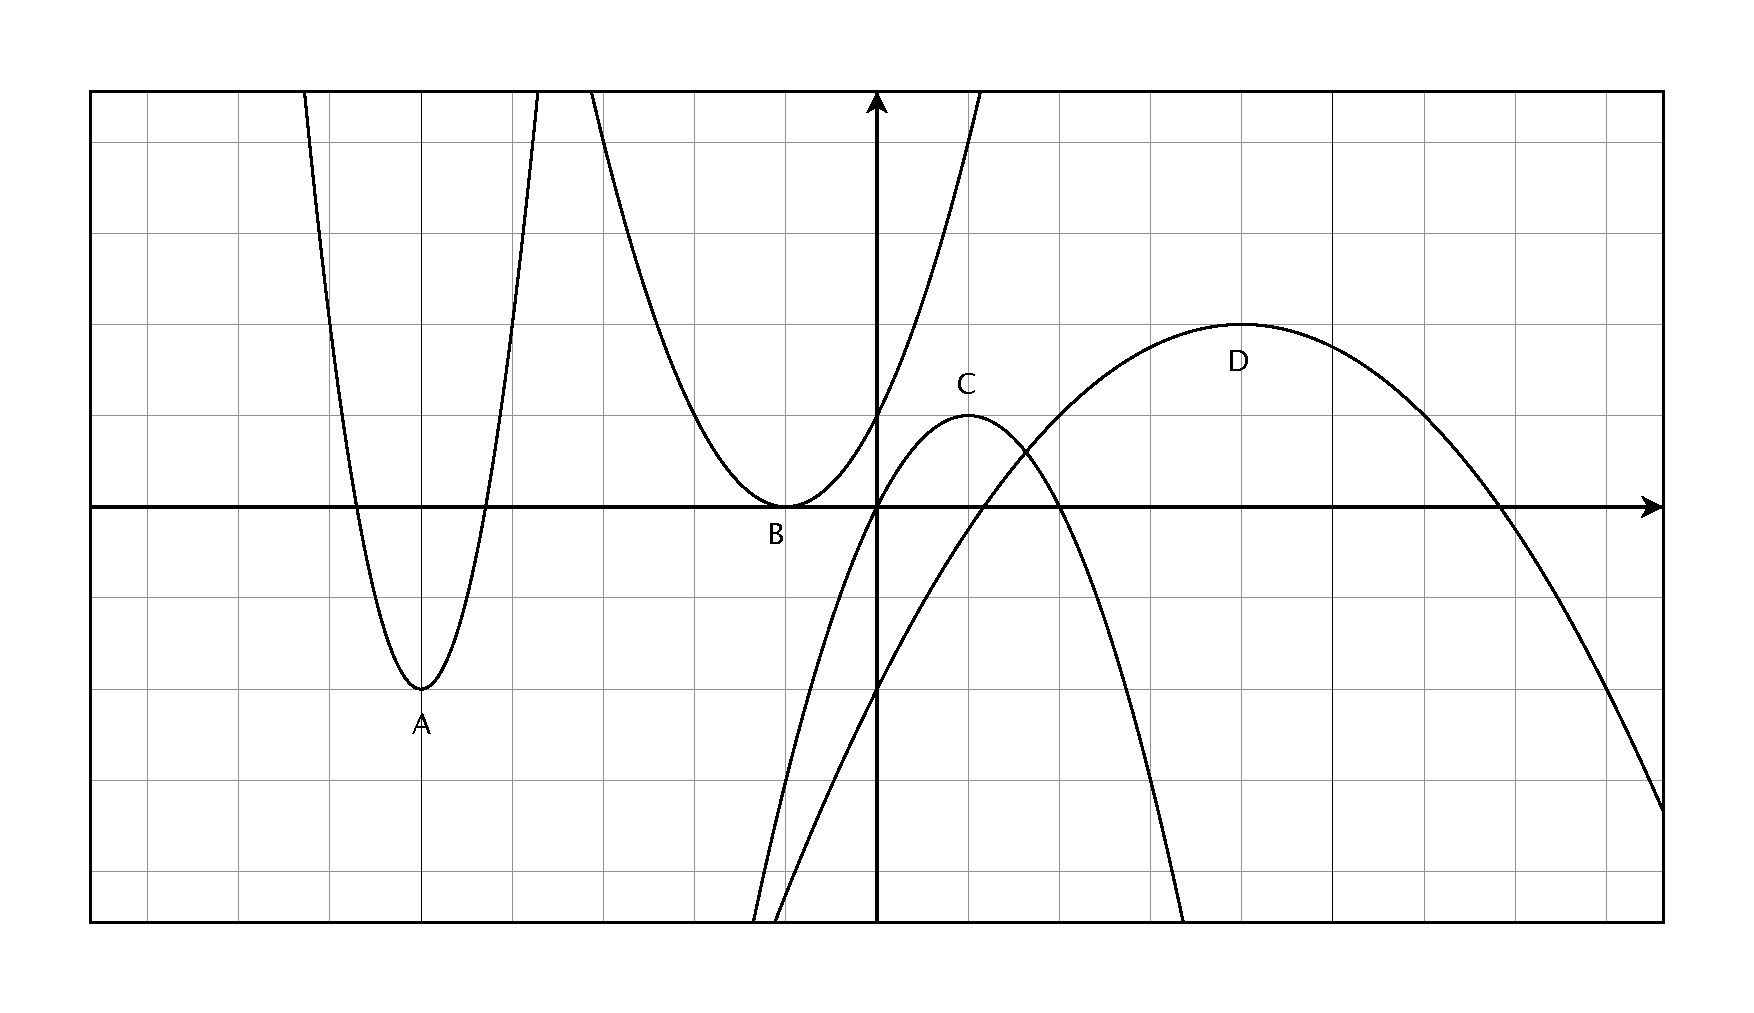
\includegraphics[scale=.3]{problem_7.eps}
%   \caption*{Problem 7}
% \end{figure}

% \begin{tabular}{cc}
% \toprule
% period & amplitude \\
% \midrule
%   $\pi$ & $2$ \\
% \bottomrule
% \end{tabular}

\title{Math 141 Notes \\ Section 4.1--Exponential Functions}

\date{June 5, 2013}

\begin{document}

  \maketitle
  \tableofcontents

  \pagebreak

  \section{Description}

  \[
    f(x) = a^x
  \]

    $a > 0$ and $a \neq 1$

  Exponentials are used when the amount of something you will have in the future is a percentage (possibly more than
  100\%) of what you have now.  
  
  Examples include bacteria growth rate, interest, and radioactive decay.

  \section{Growth Rate}
  Exponentials grow faster than polynomials because gap also grows at an exponential rate.

  \begin{itemize*}
    \item $2^x$ vs $10x$: exponential always doubles, while $f(x) = 10x$ always grows by 10
    \item $2^x$ vs $x^2$: exponential always doubles (gap is $2^x$), while $f(x) = x^2$ always grows by 1, 3, 5, $2n +
      1$.  Gap is linear and exponentials grow faster than linear.
    \item Similarly for higher degree polynomials.
  \end{itemize*}

  \begin{tabular}[h]{rrrr}
    \toprule
    $x$ & $x^2$ & $x^3$ & $2^x$ \\
    \midrule
    5  & 25    & 125     & 32 \\
    10 & 100   & 1,000   & 1,024 \\
    25 & 625   & 15,625  & 33,554,432 \\
    50 & 2,500 & 125,000 & 1,125,899,906,842,624 \\
    \bottomrule
  \end{tabular}

  P vs. NP time

  \section{Graphs}

  \begin{align*}
    f(x) &= 2^x \\
    g(x) &= \left( \frac{1}{2} \right)^x \\
         &= \left( \frac{1}{2^x} \right) \\
         &= \left( 2^{-1} \right)^x \\
         &= 2^{-x} \\
         &= f(-x) \\
  \end{align*}

  $\left( \frac{1}{2} \right)^x$ is reflection of $2^x$ around y-axis.

  Graphing examples:
  \begin{align*}
    f(x) &= 2^{x - 1} \\
    g(x) &= 2^x - 1 \\
    h(x) &= 2^{-x} \\
    i(x) &= -2^x \\
    j(x) &= -2^{-x} \\
  \end{align*}

  \pagebreak

  \begin{figure}[h]
    \centering
    \includegraphics{figure1.eps}
    \caption{$f(x) = 2 \cdot 3^x$}
    \label{fig:figure1}
  \end{figure}

  $f(x) = c \cdot a^x$ and contains: $(0, 2)$ and $(2, 18)$.  Find $c$ and $a$.

  \subsection{Compound Interest/e}

  Interest compounded annually:
  \begin{align*}
    A_1  &= P(1 + r) \\
    A_2  &= A_1(1 + r) = P(1 + r)^2 \\
    A_3  &= A_2(1 + r) = P(1 + r)^3 \\
    A(t) &= A_{t - 1}(1 + r) \\
         &= P(1 + r)^t \\
  \end{align*}

  Compounded $n$ times per year: 
  \[
    A(t) = P \left( 1 + \frac{r}{n} \right)^{nt} \\
  \]

  Compounded continuously:
  \begin{align*}
    m &= \frac{n}{r} \\
    n &= mr \\
    \\
    A(t) &= P\left(1 + \frac{r}{n}\right)^{nt} \\
         &= P\left(1 + \frac{1}{m}\right)^{mrt} \\
         &= P \left[ \left(1 + \frac{1}{m}\right)^{m} \right]^{rt} \\
    \\
    \lim_{x \to \infty} \left[ \left(1 + \frac{1}{m}\right)^{m} \right] &= e \\
  \end{align*}

  Alternate way to calculate e:
  \begin{align*}
    (1 + a)^n           &= 1 + an + a^2 \frac{n (n - 1)}{2!} + a^3 \frac{n(n-1)(n-2)}{3!} + a^4 \frac{n(n-1)(n-2)(n-3)}{4!} + \ldots \\
    (1 + \frac{1}{n})^n &= 1 + \frac{1}{n} \cdot n + \left( \frac{1}{n} \right)^2 \frac{ n (n - 1)}{2!}
        + \left( \frac{1}{n} \right)^3 \frac{n(n-1)(n-2)}{3!} + \left( \frac{1}{n} \right)^4 \frac{n(n-1)(n-2)(n-3)}{4!} + \ldots \\
        e &= 1 + 1 + \frac{1}{2!} + \frac{1}{3!} + \frac{1}{4!} + \frac{1}{5!} + \ldots \\
  \end{align*}

  e to small powers:
  \begin{align*}
    e^{1/n} &\approx \left[ \left( 1 + \frac{1}{n} \right)^n \right]^{1/n} \\
            &\approx 1 + \frac{1}{n} \\
  \end{align*}

  \section{Applications}

  \subsection{Carbon Dating}

  Amount of radioactive substance left after $t$ years:
  \[
    m(t) = m_0 e^{-kt}
  \]

  \subsection{Free Fall}

  \begin{align*}
    v(t) &= \frac{32}{k} \left( 1 - e^{-kt} \right) \\
         &\approx \frac{32}{k} \\
    y(t) &= \frac{32}{k} t + \frac{32}{k^2} e^{-kt} - \frac{32}{k^2} \\
         &\approx \frac{32}{k} t - \frac{32}{k^2} \\
  \end{align*}

  \begin{itemize*}
    \item feet and seconds
    \item $k$ depends on shape of falling object
    \item homework problem seems to be off by factor of 2 (uses 16 instead of 32)
  \end{itemize*}

  \begin{figure}[h]
    \centering
    \includegraphics[scale=0.9]{freeFallVelocity.eps}
    \caption{Free Fall Velocity ($k = 0.2$)}
  \end{figure}

  \begin{figure}[h]
    \centering
    \includegraphics[scale=0.9]{freeFallPosition.eps}
    \caption{Free Fall Position ($k = 0.2$)}
  \end{figure}
\end{document}
